\section{Handy-Eye-calibration}

The hand-eye-calibration is a current procedure to determine unknown rigid transformations, e.g. transformations between the end-effector and a tool attached to it or a transformation between the robot and the tracking system,
by taking measurements with the tracking device in different poses of the robot. For good precision and accuracy you need many different poses and they need to be linearly independent from each other. 
In this project the transformation between the robot's end-effector and the coil had to be 
determined as well as the transformation between the robots base and the coordinate system of the tracking device. The coil needed to be placed in a certain posture with respect to the head of the imaginary patient, therefore it was not enough to know only the end-effector coordinates, that can be calculated by the forward kinematics. The hand-eye-calibration uses the closed loop of four rigid transformations. That means that we can express one transformation or a combination of two, by means of the remaining ones. Two of these transformations are fixed and the other two can vary. \figref{handeye} shows the installation.

\begin{figure}[!t]
	\centering 
		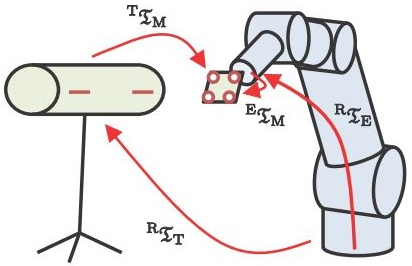
\includegraphics[width=3.5in]{handeye.JPG}		
			\caption{Hand-Eye-calibration setup} 
			\label{handeye} 
\end{figure}

\begin{equation}
	M = ^RT_E
\end{equation}

\begin{equation}
	X = ^ET_M
\end{equation}
	
\begin{equation}
	N = ^TT_M
\end{equation}
	
\begin{equation}
	Y = ^RT_T
\end{equation}

We are interested in the fixed ones $^E$T$_M$ and $^R$T$_T$ whereas the variable ones can be calculated or measured. We can write \\

\begin{equation}
	M \cdot X = Y \cdot N
\end{equation}

or 

\begin{equation}
	M_i \cdot X = N_i \cdot Y
\end{equation}

where index $i$ denotes one set of measurements. 

These equations can be rearranged and written as 

\begin{equation}
	A \cdot w = b
\end{equation}

where $A$ and $b$ contain manipulated values of $M_i$ and $N_i$, so that we can fill these matrices with 
actual measurement values to calculate $w$. After the calculation the solution vector $w$, it contains the
24 not trivial values of $X$ and $Y$. The last step of the calibration is to orthonormalize $X$ and $Y$
since the calculation of $w$ provides independant values for the rotation and translation. 
If the translation can be taken as given, the vectors of the rotation matrix need to be orthonormal \cite{ref:hand_eye_calib_paper}.